\documentclass[aspectratio=169,12pt]{beamer}

% ---- Theme ----
\usetheme{Madrid}
\usecolortheme{seahorse}
\setbeamertemplate{navigation symbols}{}
\setbeamertemplate{footline}[frame number]
\setbeamertemplate{itemize items}[circle]
\setbeamersize{text margin left=8mm,text margin right=8mm}

% ---- Packages ----
\usepackage{amsmath,amssymb}
\usepackage{graphicx}
\usepackage{booktabs}
\usepackage{tikz}
\usetikzlibrary{positioning,arrows.meta,shapes.geometric}
\usepackage{xcolor}

% ---- Custom colors ----
\definecolor{waterdark}{RGB}{0,70,120}
\definecolor{waterlight}{RGB}{135,195,225}
\definecolor{accent}{RGB}{200,60,50}
\definecolor{dimgray}{RGB}{120,120,120}

\setbeamercolor{title}{fg=waterdark}
\setbeamercolor{frametitle}{fg=waterdark}
\setbeamercolor{structure}{fg=waterdark}
\setbeamercolor{alerted text}{fg=accent}

% ---- Macros ----
\newcommand{\source}[1]{\vfill\hfill{\tiny\textcolor{dimgray}{#1}}}

% ===========================================================================
\begin{document}
% ===========================================================================

% ---------- TITLE ----------
\begin{frame}
\vspace{1.5cm}
\begin{center}
{\Large\color{waterdark}\textbf{The Economics of Water Scarcity}}\\[6pt]
{\normalsize Internal Specification-Sensitivity Analysis of the\\Water Scarcity--GDP Growth Estimate}\\[16pt]
{\small Augusto Gonzalez-Bonorino}\\[4pt]
{\footnotesize ECN 726 $\cdot$ Arizona State University $\cdot$ April 2026}
\end{center}
\vfill
{\footnotesize Replicating: Frost, Madeira \& Martinez Jaramillo (2025), ``The Economics of Water Scarcity,'' BIS WP 1314.}
\end{frame}

% ---------- SLIDE 1: WHY WATER? ----------
\begin{frame}{Why Should Economists Care About Water?}

\begin{columns}[T]
\begin{column}{0.55\textwidth}
\vspace{0.3cm}
Water is a \alert{universal input}:
\begin{itemize}
    \item Agriculture (70\% of global withdrawals)
    \item Energy generation (cooling, hydro)
    \item Industry and services
    \item Household consumption
\end{itemize}

\vspace{0.4cm}
Yet water is \alert{chronically underpriced}:
\begin{itemize}
    \item Subsidies suppress marginal cost signals
    \item Agriculture pays $<$\$2.50/m\textsuperscript{3} everywhere
    \item $\Rightarrow$ Overuse, underinvestment, tragedy of the commons
\end{itemize}
\end{column}

\begin{column}{0.42\textwidth}
\vspace{0.2cm}
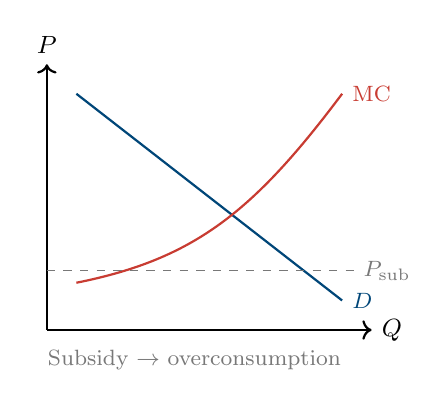
\begin{tikzpicture}[scale=0.75, every node/.style={font=\small}]
    % Axes
    \draw[->,thick] (0,0) -- (5.5,0) node[right] {$Q$};
    \draw[->,thick] (0,0) -- (0,4.5) node[above] {$P$};
    % Demand
    \draw[thick,waterdark] (0.5,4) -- (5,0.5) node[right,font=\footnotesize] {$D$};
    % MC (true)
    \draw[thick,accent] (0.5,0.8) .. controls (2.5,1.2) and (3.5,2) .. (5,4) 
        node[right,font=\footnotesize] {MC};
    % Subsidized price
    \draw[dashed,dimgray] (0,1.0) -- (5.2,1.0) node[right,font=\footnotesize] {$P_{\text{sub}}$};
    % Labels
    \node[font=\footnotesize,dimgray] at (2.5,-0.5) {Subsidy $\to$ overconsumption};
\end{tikzpicture}
\end{column}
\end{columns}

\source{OECD (2010); Frost et al.\ (2025) Graph 6, Graph A.2}
\end{frame}

% ---------- SLIDE 2: DATA ----------
\begin{frame}{Data: A Global Panel}

\begin{columns}[T]
\begin{column}{0.48\textwidth}
\textbf{Panel structure}
\begin{itemize}
    \item 169 countries, 1990--2020
    \item Unbalanced panel ($N \approx 4{,}583$)
    \item Water data: FAO Aquastat\\(collected $\sim$every 5 years, interpolated)
\end{itemize}

\vspace{0.3cm}
\textbf{Key variables}
\begin{itemize}
    \item $Y$: Annual real GDP growth (\%)
    \item $W^{pc}$: Water withdrawal per capita
    \item $WS$: Freshwater withdrawal / available resources (\%)
    \item $\text{GDP}^{pc}$: Income at PPP
\end{itemize}
\end{column}

\begin{column}{0.48\textwidth}
\vspace{0.2cm}
\centering
{\small\textbf{Summary Statistics}}\\[4pt]
\begin{tabular}{lcc}
\toprule
& Median & SD \\
\midrule
GDP growth (\%) & 4 & 6 \\
Scarcity (\%) & 7--12 & 29--33 \\
$\ln(W^{pc})$ & 5.8 & 1.2 \\
$\ln(\text{GDP}^{pc})$ & 9.2 & 1.2 \\
\bottomrule
\end{tabular}

\vspace{0.5cm}
{\footnotesize Right-skewed scarcity: medians 7--12\% but means 21--28\% $\Rightarrow$ long tail of water-stressed countries.}
\end{column}
\end{columns}

\source{Frost et al.\ (2025), Table 2}
\end{frame}

% ---------- SLIDE 3: MODEL ----------
\begin{frame}{Theoretical Model: Water in Production}

\textbf{Modified Cobb-Douglas} with water as a factor:
\[
Y_{ct} = \mathit{TFP}_{ct} \cdot \bigl[\underbrace{g(W,WS)}_{\text{effective water}}\bigr]^{1-\alpha-\theta} \cdot [K^p(W)]^{\alpha} \cdot [L \cdot h(W)]^{\theta}
\]

\pause
\vspace{0.1cm}
\textbf{Why both $W$ \emph{and} $WS$?}
\begin{itemize}
    \item $W$ = volume of water used (input quantity)
    \item $WS$ = withdrawal / available resources (scarcity pressure)
    \item $g(W, WS) = \dfrac{W}{1 + WS}$\quad --- scarcity \alert{discounts} the effective water input
\end{itemize}

\pause
\vspace{0.2cm}
\textbf{Role of $g(\cdot)$}: captures \emph{decreasing marginal productivity} of water as scarcity rises. Even with the same withdrawal $W$, a country at 80\% scarcity gets less ``effective water'' than one at 10\%.

\source{Frost et al.\ (2025), Equations 1--2}
\end{frame}

% ---------- SLIDE 4: ESTIMATION ----------
\begin{frame}{From Theory to Estimation}

Log-linearize $\to$ approximate $\ln(1+WS) \approx WS$ for small scarcity $\to$ panel regression:

\vspace{0.2cm}
\[
\boxed{\;\Delta\ln Y_{ct} = \beta_1 \ln(W^{pc}_{ct}) + \beta_2\, WS_{ct} + \beta_3 \ln(\text{GDP}^{pc}_{ct}) + \alpha_c + \alpha_t + \varepsilon_{ct}\;}
\]

\vspace{0.3cm}
\begin{columns}[T]
\begin{column}{0.48\textwidth}
\textbf{Identification strategy}
\begin{itemize}
    \item Country FE: absorb geography, institutions
    \item Year FE: absorb global shocks
    \item SE clustered by country
\end{itemize}
\end{column}
\begin{column}{0.48\textwidth}
\textbf{Key caveats}
\begin{itemize}
    \item Association, not causation
    \item Linear approx.\ poor at high scarcity
    \item Interpolated water data attenuates FE signal
\end{itemize}
\end{column}
\end{columns}

\vspace{0.3cm}
\centering
\alert{Focal metric}: $\hat{\beta}_2 = -0.102^{***}$ \quad (SE $= 0.039$, $N = 4{,}583$)

\source{Frost et al.\ (2025), Table 3 col.\ 3}
\end{frame}

% ---------- SLIDE 5: SOURCE PAPER RESULTS ----------
\begin{frame}{Source Paper: Key Results}

\begin{center}
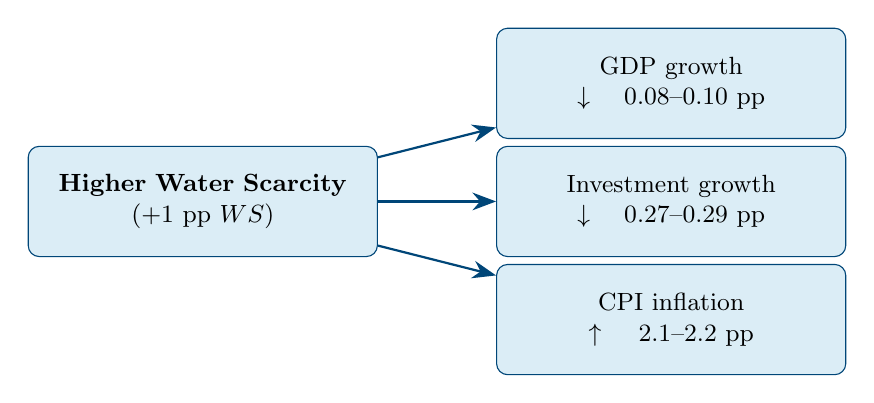
\begin{tikzpicture}[
    node distance=0.6cm,
    block/.style={rectangle, rounded corners, draw=waterdark, fill=waterlight!30,
        text width=4.2cm, minimum height=1.4cm, align=center, font=\small},
    arrow/.style={-{Stealth[length=3mm]}, thick, waterdark}
]
    \node[block] (ws) {\textbf{Higher Water Scarcity}\\($+1$ pp $WS$)};
    \node[block, right=1.5cm of ws, yshift=1.5cm] (gdp) {GDP growth\\$\downarrow\; 0.08$--$0.10$ pp};
    \node[block, right=1.5cm of ws] (inv) {Investment growth\\$\downarrow\; 0.27$--$0.29$ pp};
    \node[block, right=1.5cm of ws, yshift=-1.5cm] (cpi) {CPI inflation\\$\uparrow\; 2.1$--$2.2$ pp};
    
    \draw[arrow] (ws) -- (gdp);
    \draw[arrow] (ws) -- (inv);
    \draw[arrow] (ws) -- (cpi);
\end{tikzpicture}
\end{center}

\vspace{0.2cm}
\begin{itemize}
    \item Consistent across 3 scarcity measures (internal, renewable, available)
    \item Quantile regressions: strongest negative effect at \alert{Q25} (low-growth episodes)
    \item Water use \emph{efficiency} positively associated with GDP growth;\\effect fades for higher-income countries
\end{itemize}

\source{Frost et al.\ (2025), Tables 3--6, Table A.4}
\end{frame}

% ---------- SLIDE 6: MY FOCUS ----------
\begin{frame}{My Focus: How Robust is $\hat{\beta}_2 = -0.102$?}

\begin{columns}[T]
\begin{column}{0.55\textwidth}
\textbf{Motivating questions}
\begin{itemize}
    \item The baseline is \emph{one} specification among many plausible alternatives
    \item Does the sign hold across modeling choices?
    \item Does the magnitude survive?
    \item Which decisions matter most?
\end{itemize}

\vspace{0.3cm}
\textbf{Two empirical hints}
\begin{itemize}
    \item Q25 effect $>$ Q75 effect $\Rightarrow$ possible \alert{nonlinearity}
    \item Scarcity and income are correlated $\Rightarrow$ possible \alert{heterogeneity} by development level
\end{itemize}
\end{column}

\begin{column}{0.42\textwidth}
\vspace{0.3cm}
\centering
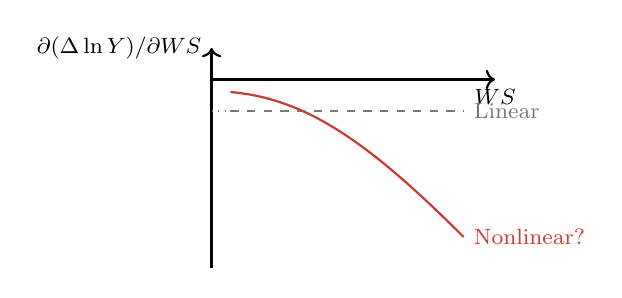
\begin{tikzpicture}[scale=0.8]
    \draw[->,thick] (0,0) -- (4.5,0) node[below,font=\footnotesize] {$WS$};
    \draw[->,thick] (0,-3) -- (0,0.5) node[left,font=\footnotesize] {$\partial(\Delta\ln Y)/\partial WS$};
    % Linear
    \draw[thick,dimgray,dashed] (0.3,-0.5) -- (4,-0.5) 
        node[right,font=\footnotesize,dimgray] {Linear};
    % Nonlinear
    \draw[thick,accent] (0.3,-0.2) .. controls (1.5,-0.3) and (2.5,-1) .. (4,-2.5) 
        node[right,font=\footnotesize,accent] {Nonlinear?};
    \draw[dotted,dimgray] (0,-0.5) -- (0.3,-0.5);
\end{tikzpicture}

\vspace{0.3cm}
{\footnotesize Does the marginal growth penalty increase with scarcity?}
\end{column}
\end{columns}

\source{Banzhaf \& Smith (2007); Simonsohn et al.\ (2020)}
\end{frame}

% ---------- SLIDE 7: META-ANALYSIS DESIGN ----------
\begin{frame}{Specification-Sensitivity Analysis: Design}

\begin{center}
$\underbrace{3}_{\text{Scarcity measures}} \;\times\; \underbrace{5}_{\text{Functional forms}} \;\times\; \underbrace{8}_{\text{Estimators}} \;=\; \alert{120}$ \text{ specifications}
\end{center}

\vspace{0.2cm}

\begin{columns}[T]
\begin{column}{0.30\textwidth}
\textbf{Scarcity measure}\\[4pt]
{\small
\begin{enumerate}
    \item Internal resources
    \item Total renewable
    \item Available freshwater
\end{enumerate}
}
\end{column}

\begin{column}{0.35\textwidth}
\textbf{Functional form}\\[4pt]
{\small
\begin{enumerate}
    \item Linear (baseline)
    \item Quadratic
    \item $WS \times \ln(\text{GDP}^{pc})$
    \item $WS \times \ln(W^{pc})$
    \item Piecewise threshold
\end{enumerate}
}
\end{column}

\begin{column}{0.32\textwidth}
\textbf{Estimator}\\[4pt]
{\small
\begin{enumerate}
    \item Country FE only
    \item Two-way FE
    \item Random effects
    \item Between
    \item First differences
    \item Quantile Q25
    \item Quantile Q50
    \item Quantile Q75
\end{enumerate}
}
\end{column}
\end{columns}

\vspace{0.3cm}
\centering
{\small Meta-regression: $\hat{\beta}_s = \gamma_0 + \sum_j \gamma_j\, d_{j,s} + \varepsilon_s$\quad (omitted: linear, available FW, two-way FE)}

\source{Following Banzhaf \& Smith (2007) internal meta-analysis methodology}
\end{frame}

% ---------- SLIDE 8: SPEC CURVE ----------
\begin{frame}{Results: Specification Curve}

\begin{center}
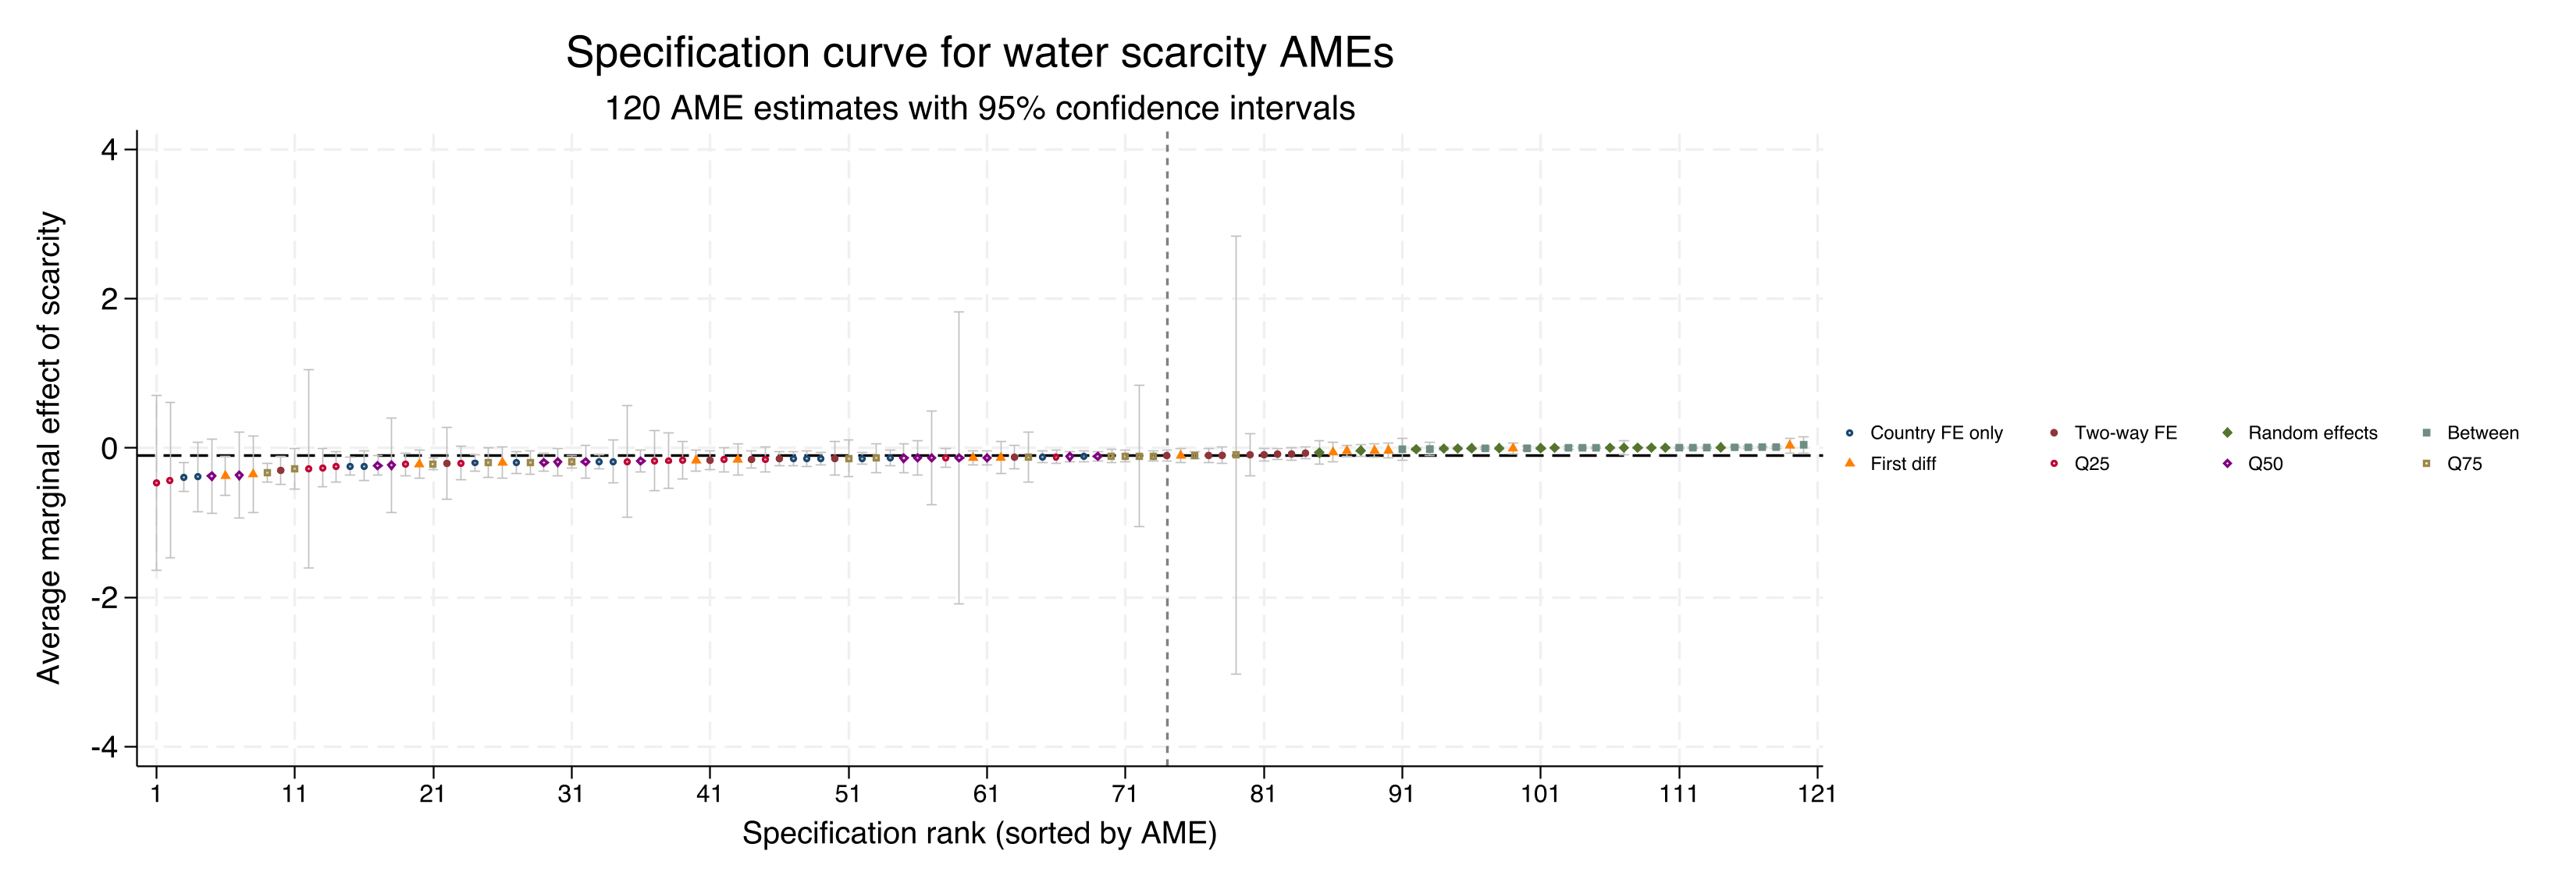
\includegraphics[width=0.9\textwidth]{../figures/fig_spec_curve.png}
\end{center}

\vspace{-0.2cm}
{\footnotesize 120 AME estimates sorted by magnitude. Dashed line = replicated baseline ($-0.102$). Color = estimator. The companion decision-matrix figure is exported separately.}

\end{frame}

% ---------- SLIDE 9: DISTRIBUTION ----------
\begin{frame}{Results: Distribution of 120 Estimates}

\begin{center}
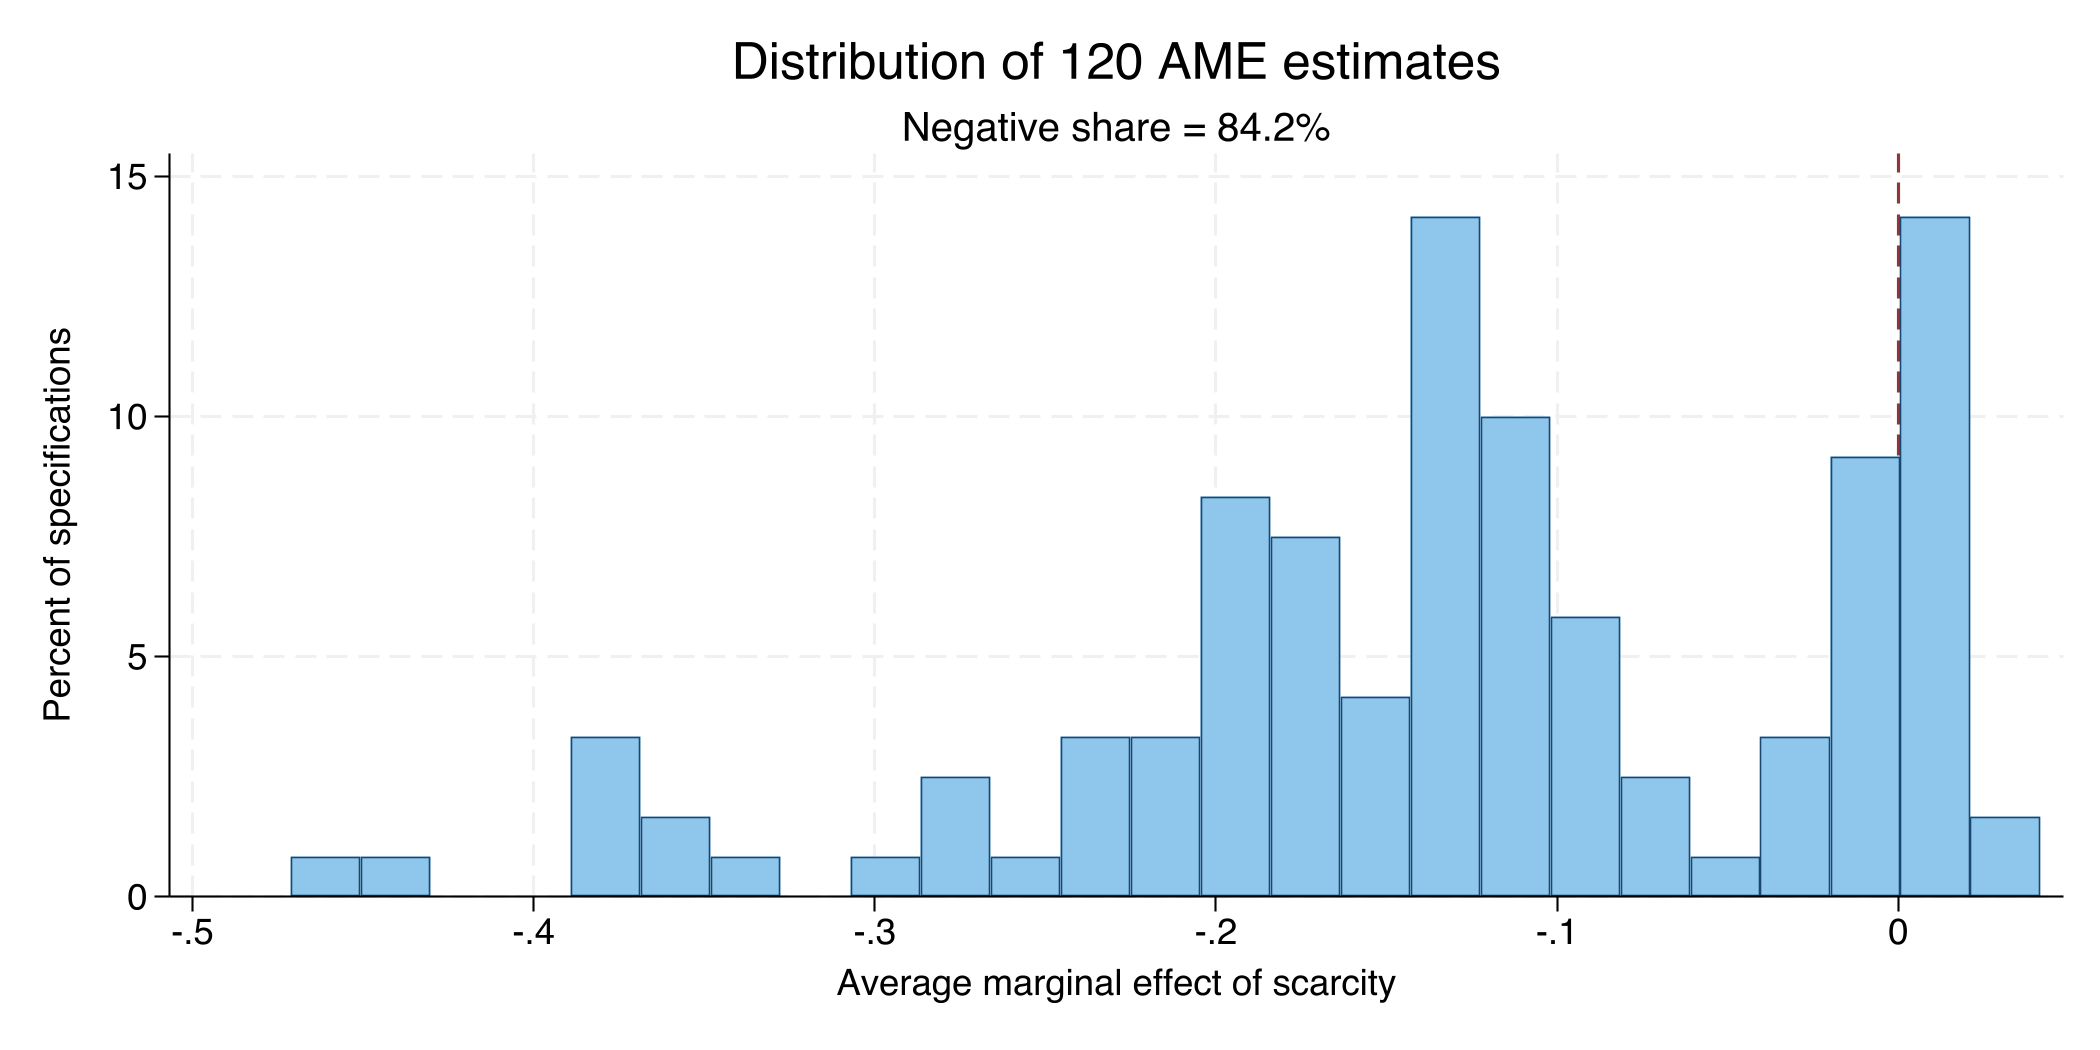
\includegraphics[width=0.78\textwidth]{../figures/fig_histogram.png}
\end{center}

\vspace{-0.2cm}
{\footnotesize Mean AME $=-0.129$, median $=-0.131$, IQR $=[-0.187,-0.025]$, 84.2\% negative, 39.2\% significant at 5\%. The sign is stable; the magnitude is not.}

\end{frame}

% ---------- SLIDE 10: META-REGRESSION ----------
\begin{frame}{Results: What Drives the Variation?}

\begin{columns}[T]
\begin{column}{0.55\textwidth}
\begin{center}
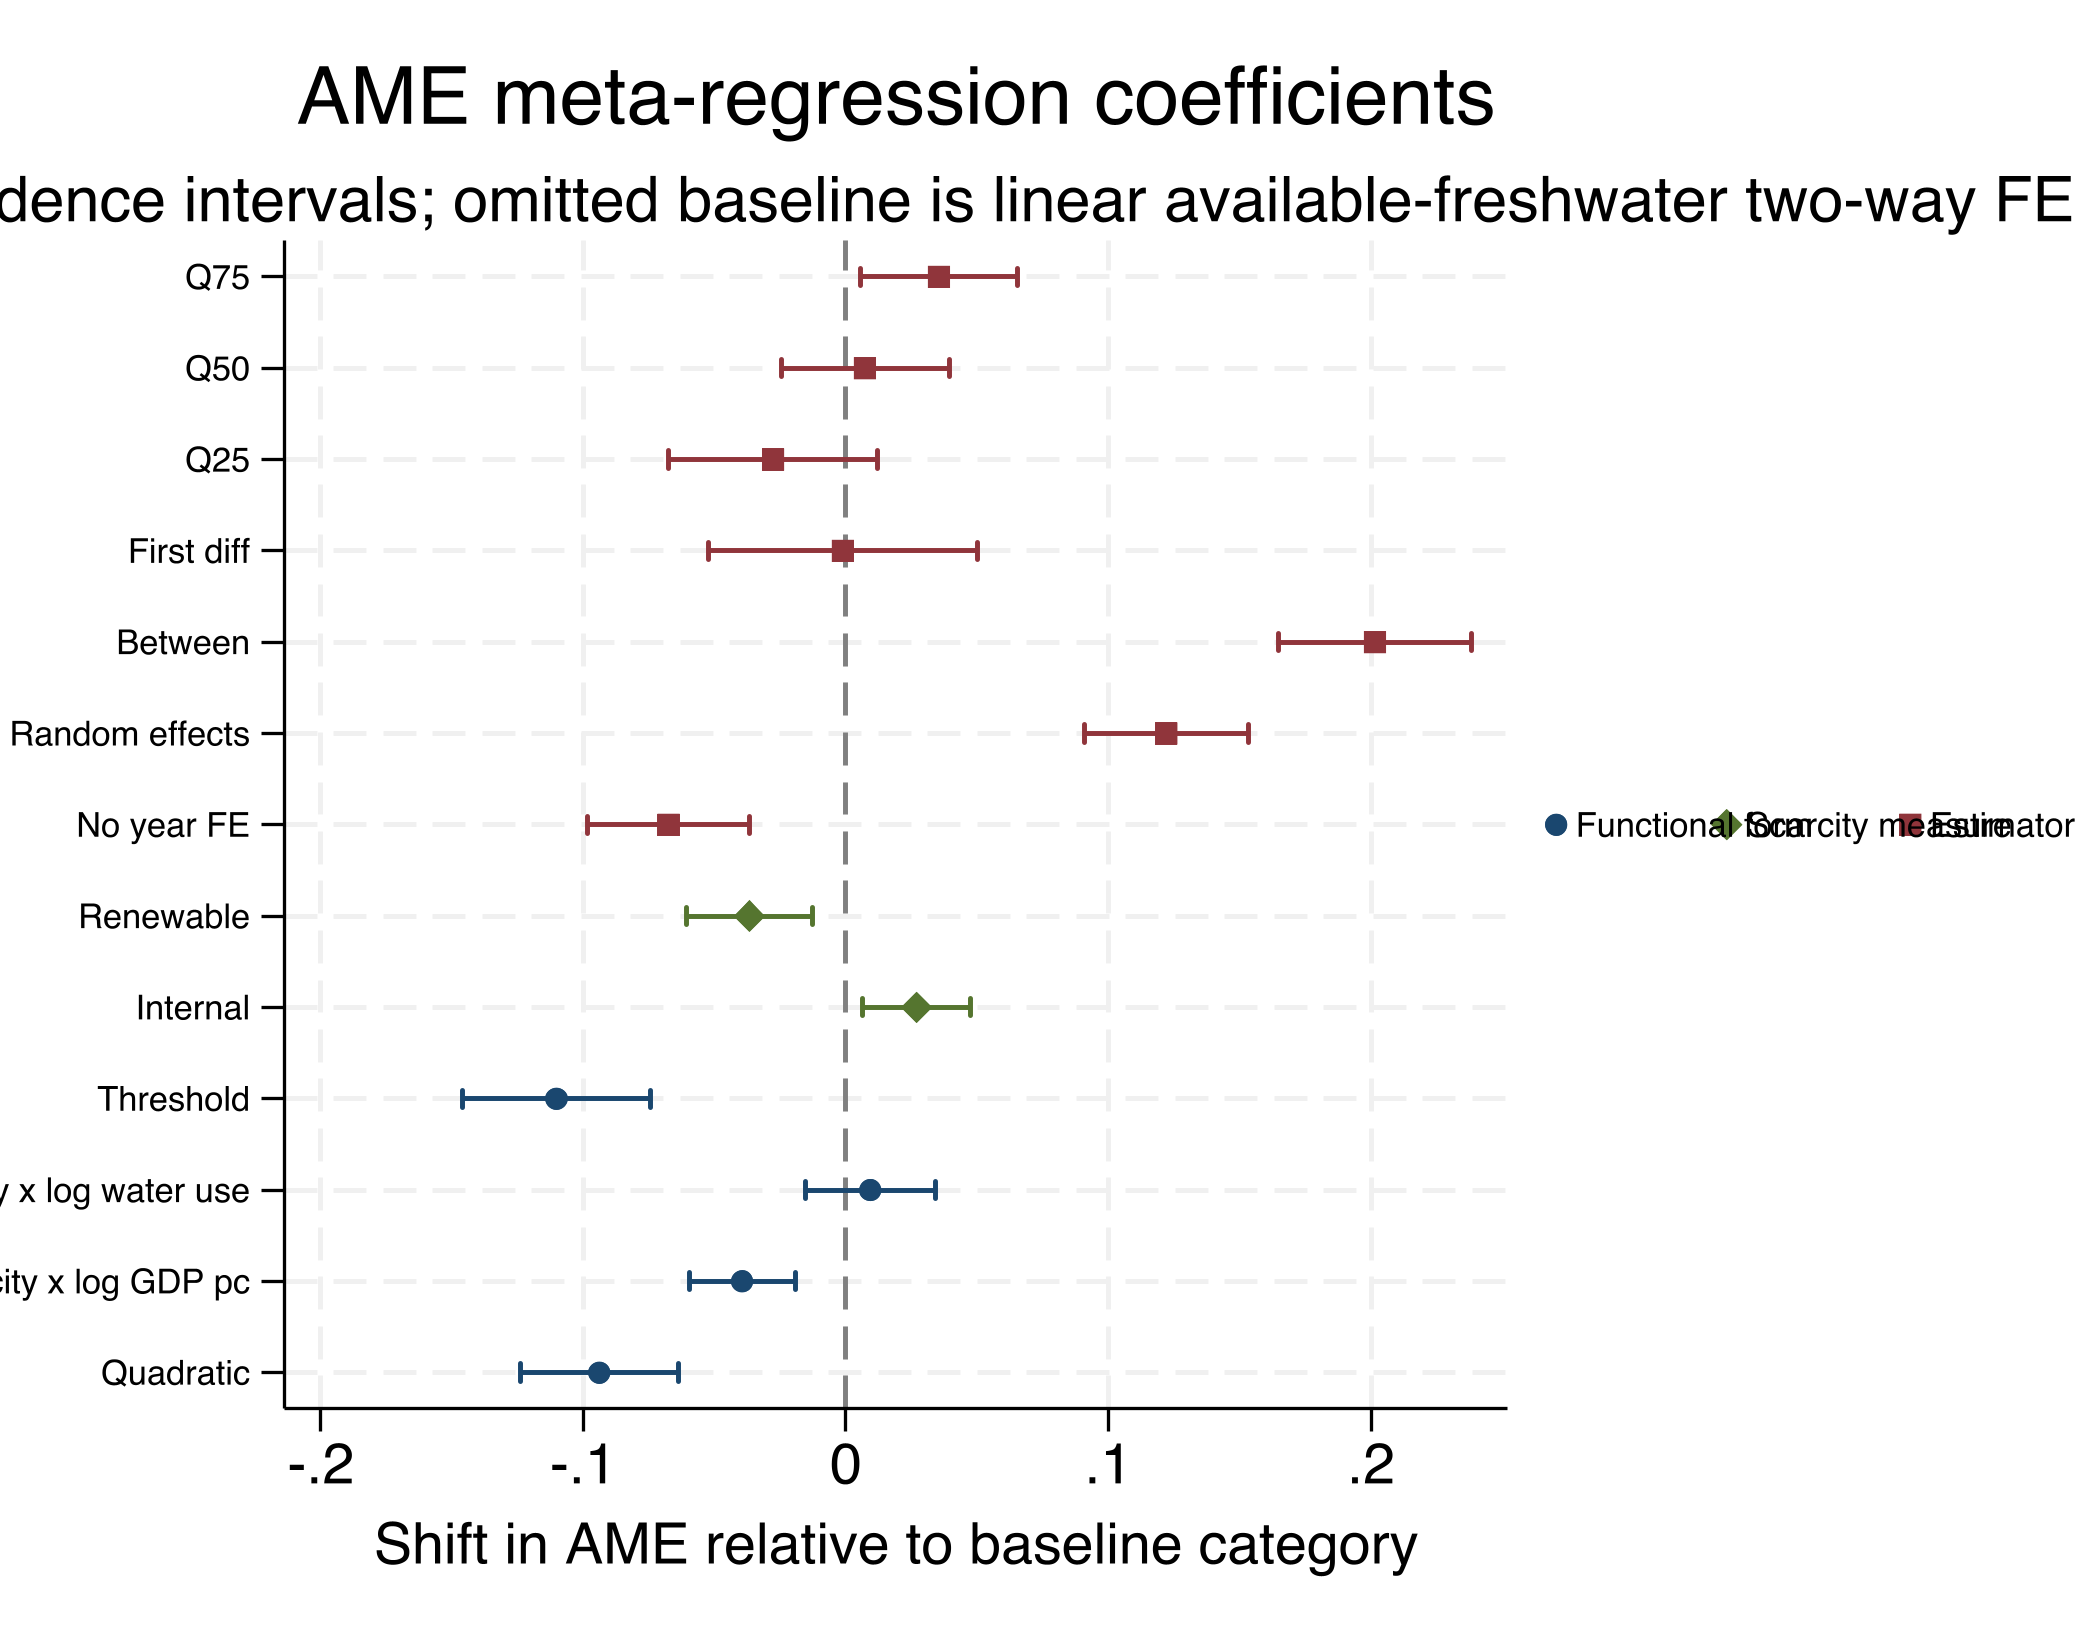
\includegraphics[width=\textwidth]{../figures/fig_coef_plot.png}
\end{center}
\end{column}

\begin{column}{0.42\textwidth}
\vspace{0.1cm}
\textbf{Three findings:}

\vspace{0.2cm}
\alert{1. Functional form still matters}
\begin{itemize}
    \item[\footnotesize$\bullet$] {\small Quadratic and threshold forms shift AMEs further negative}
    \item[\footnotesize$\bullet$] {\small Income interaction remains more negative on average after AME correction}
\end{itemize}

\vspace{0.2cm}
\alert{2. Year effects matter}
\begin{itemize}
    \item[\footnotesize$\bullet$] {\small No-year-FE penalty is clearly negative}
    \item[\footnotesize$\bullet$] {\small Dropping common time shocks makes scarcity look worse}
\end{itemize}

\vspace{0.2cm}
\alert{3. Tail sensitivity remains}
\begin{itemize}
    \item[\footnotesize$\bullet$] {\small Q25 is the most negative quantile shift}
    \item[\footnotesize$\bullet$] {\small Q50 is near zero and Q75 turns positive relative to Q25}
\end{itemize}
\end{column}
\end{columns}

\source{AME-based meta-regression with HC1 standard errors; coefficients relative to the linear / available-freshwater / two-way-FE baseline}
\end{frame}

% ---------- SLIDE 11: CONCLUSION ----------
\begin{frame}{Conclusions}

\textbf{On the robustness of the source paper:}
\begin{itemize}
    \item The \alert{direction} of the scarcity--growth association is stable (84.2\% negative)
    \item The \alert{magnitude} is sensitive --- especially to functional form and estimator
    \item The linear baseline may understate heterogeneity: the interaction plot shows attenuation with income, not invariance
\end{itemize}

\vspace{0.3cm}
\textbf{Policy implications:}
\begin{itemize}
    \item Pricing reform: move toward marginal-cost pricing to reduce overuse\\{\footnotesize(OECD 2010: most tariffs provide little incentive for efficiency)}
    \item Infrastructure investment: poorer countries lack the buffers that richer countries use to mitigate scarcity
    \item Monitoring: water scarcity deserves attention alongside energy and climate in macro forecasting
\end{itemize}

\end{frame}

% ---------- SLIDE 12: DISCUSSION ----------
\begin{frame}{Discussion: Should We Study Water More?}

\vspace{0.3cm}

\begin{quote}
{\small ``Reliable data for water use at the industry level has not been obtained since 1982.''}\\
\hfill --- Basker et al.\ (2019)
\end{quote}

\vspace{0.4cm}

\textbf{Open questions for economists:}
\begin{itemize}
    \item Is there a standard model of water as an economic object?\\
    {\small Used in production \emph{and} consumption, with pervasive externalities}
    \item What does it mean to put $W$ and $WS$ in a Cobb-Douglas?\\
    {\small $g(\cdot)$ acts as a technology wedge --- is this a new form of ``capital''?}
    \item Can we identify a \emph{causal} effect?\\
    {\small IV from rainfall variation? Upstream dam construction?}
    \item Water scarcity is projected to worsen under climate change ---\\should central banks and macro forecasters be paying attention?
\end{itemize}

\vspace{0.3cm}
\centering
{\large\color{waterdark}\textbf{Thank you. Questions?}}

\end{frame}

\end{document}
